\documentclass{standalone}
\usepackage{tikz}
\usepackage{ctex,siunitx}
\setCJKmainfont{Noto Serif CJK SC}
\usepackage{tkz-euclide}
\usepackage{amsmath}
\usetikzlibrary{patterns, calc}
\usetikzlibrary {decorations.pathmorphing, decorations.pathreplacing, decorations.shapes,}

\begin{document}
\small
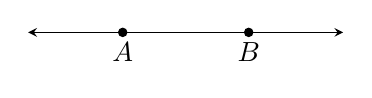
\begin{tikzpicture}[>=stealth,scale=1.0]
  \tkzSetUpPoint[fill=black]
  % \useasboundingbox(-1,-0.75)rectangle(3.7,1.4);
  \draw[<->](-2,1)--(2,1);
  \draw (-.8,1) [fill=black]circle (1.5pt)node[below]{$A$};
  \draw (.8,1) [fill=black]circle (1.5pt)node[below]{$B$};
\end{tikzpicture}
\end{document}